\chapter[Tau leptons][Tau leptons]{Tau leptons}
\label{chap:taus}

\begin{quote}
  Tau leptons and their signature in the ATLAS detector are described. 
\end{quote}

% ----------------------------------------------------------------------------------

\section{Tau leptons}
\label{sec:taus-theory}

Tau leptons were discovered in the 1970s by Martin Perl and the SLAC-LBL group at the SPEAR electron-positron collider~\cite{1975.Perl.discovery_of_tau_1,1976.Perl.discovery_of_tau_2,1977.Perl.discovery_of_tau_3}. They have since been studied in great detail at experiments like Belle~\cite{todo} and BaBar~\cite{todo}. The associated tau neutrino was first observed directly at the DONUT experiment in 2000~\cite{todo}, though its existence was inferred by measurements of the width of the $Z$ boson by experiments at the LEP collider in 1990~\cite{todo,todo}.

Tau leptons are the heaviest of the charged leptons. Their mass of 1.78 GeV is approximately twenty times larger than the muon mass~\cite{todo}, and their short lifetime $c\tau = \text{87 } \mu m$ implies tau leptons produced in $pp$ collisions at the LHC typically decay within the ATLAS beam pipe. The ATLAS detector therefore observes only the decay products of the tau lepton, not the particle itself.

Tau leptons decay leptonically ($\tauldecay$) in 35\% of decays and hadronically ($\tauhdecay$) in 65\%. Among hadronic decays, 72\% involve exactly one charged pion and 22\% exactly three charged pions. The remaining percentage of hadronic decays dominantly involves kaons or five (or more) charged pions. All tau lepton decays involve at least one neutrino. A pie chart of tau lepton branching fraction is given in \cref{fig:taus-decaypie}.

\begin{figure}[tp]
  \centering
  \includegraphics[width=0.48\textwidth]{figures/piecharts/taudecay}
  \caption{Variables.}
  \label{fig:taus-decaypie}
\end{figure}

% ----------------------------------------------------------------------------------

\section{Leptonic tau decays, $\taul$}
\label{sec:taus-leptons}

At ATLAS, light leptons from tau lepton decays ($\tauldecay$) are largely indistinguishable from prompt leptons from $W$ and $Z$ decays. They are typically less energetic due to the presence of two additional neutrinos in the tau lepton decay (e.g., $\Wlv$ versus $\Wtauvlvvv$), but for identification purposes, the only distinguishing features arise from the displaced tau vertex. This displacement is often quantified by the transverse distance of closest approach $d_0$ of the light lepton to the production (``primary'') vertex. But given the short lifetime of tau leptons, the discrimination power is weak. These properties are demonstrated in \cref{fig:taus-leptonpt}.

\begin{figure}[tp]
  \centering
  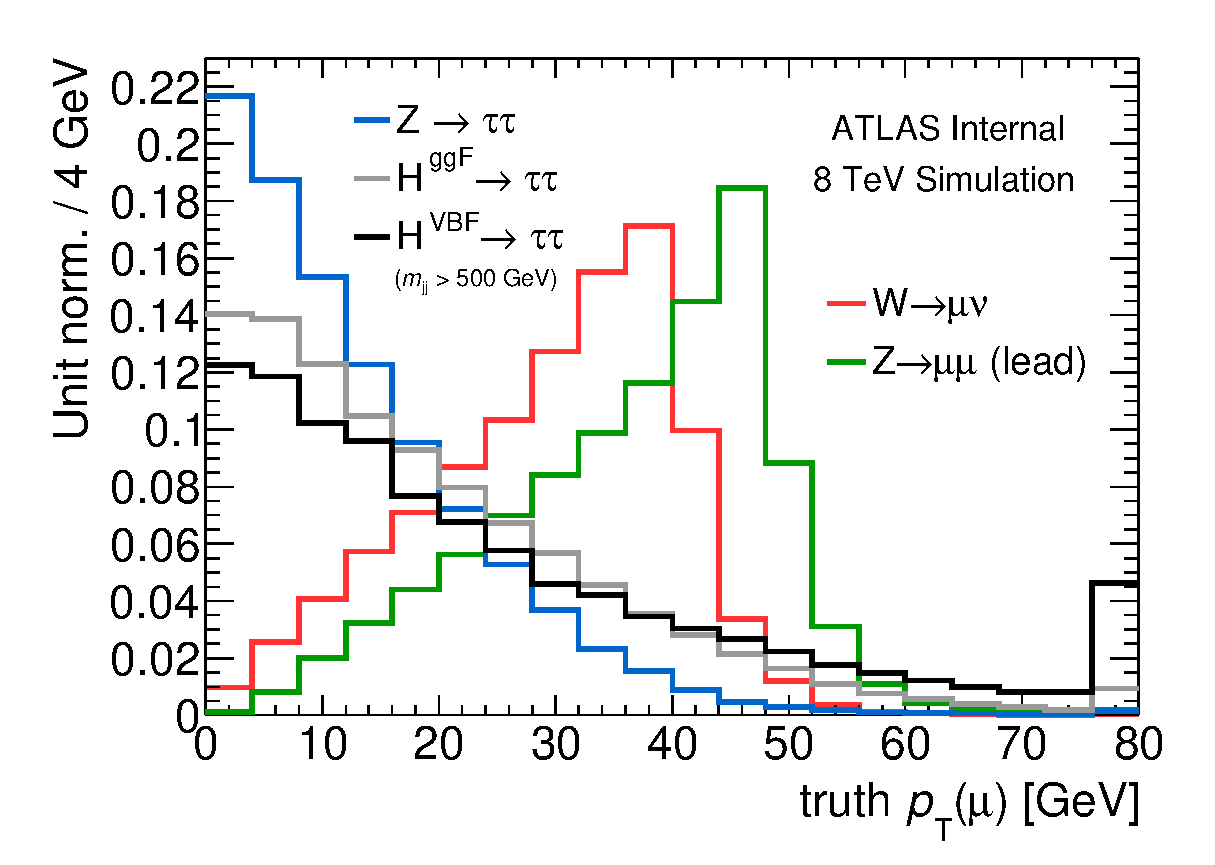
\includegraphics[width=0.48\textwidth]{figures/tauperformance/leptonsfromtausaresoft}
  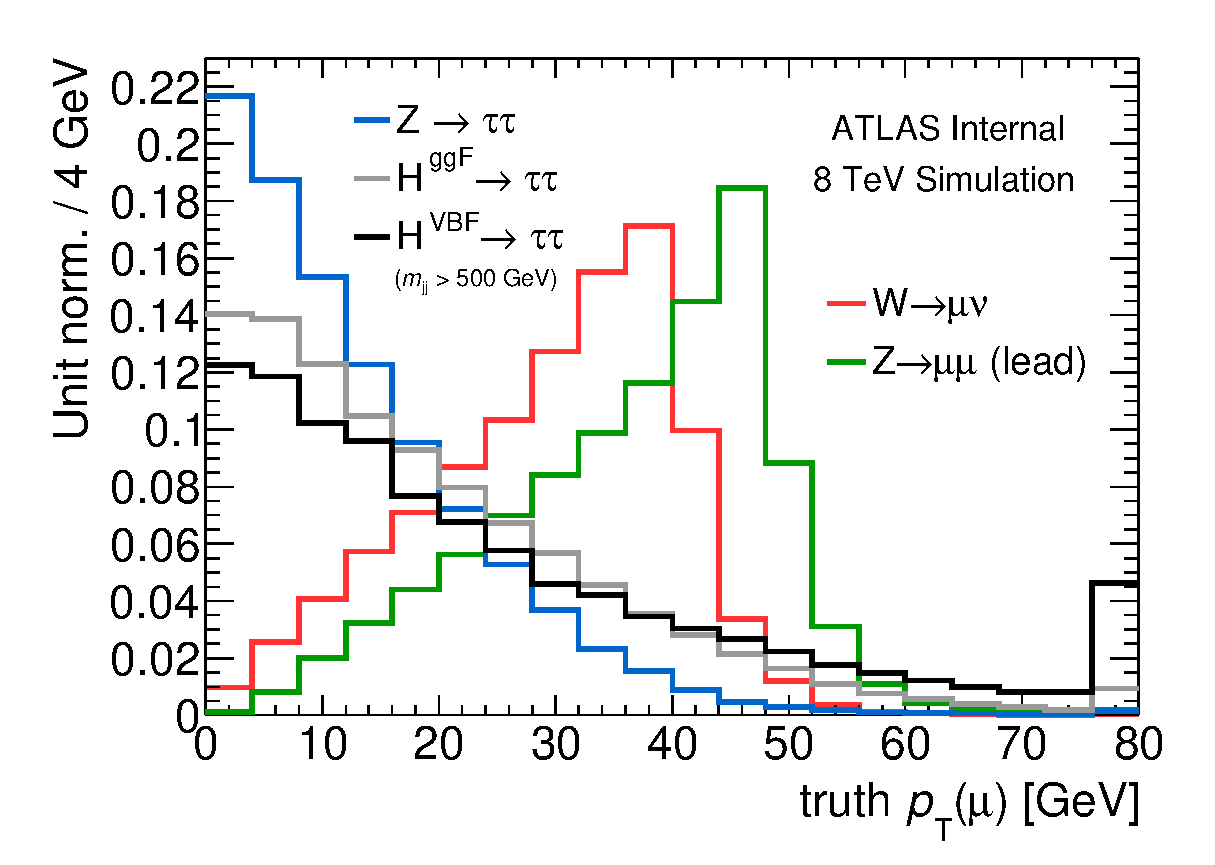
\includegraphics[width=0.48\textwidth]{figures/tauperformance/leptonsfromtausaresoft}
  \caption{True $\pt$ and reconstructed $d_0$ for muons from simulated $W$, $Z$, and tau lepton decays. Muons from tau lepton decays are shown for $\Ztautau$, $\ggFHtautau$, and $\VBFHtautau$ processes.}
  \label{fig:taus-leptonpt}
\end{figure}

% ----------------------------------------------------------------------------------

\section{Hadronic tau decays, $\tauh$}
\label{sec:taus-jetfakes}

\subsection{Reconstruction}
\subsection{Calibration}
\subsection{Identification}

\begin{figure}[tp]
  \centering
  \includegraphics[width=0.95\textwidth]{figures/tauperformance/vp1_3dcocktail_run182424_evt2582762_tttaumu}
  \caption{Variables.}
  \label{fig:taus-eventdisplay}
\end{figure}

\begin{figure}[tp]
  \centering
  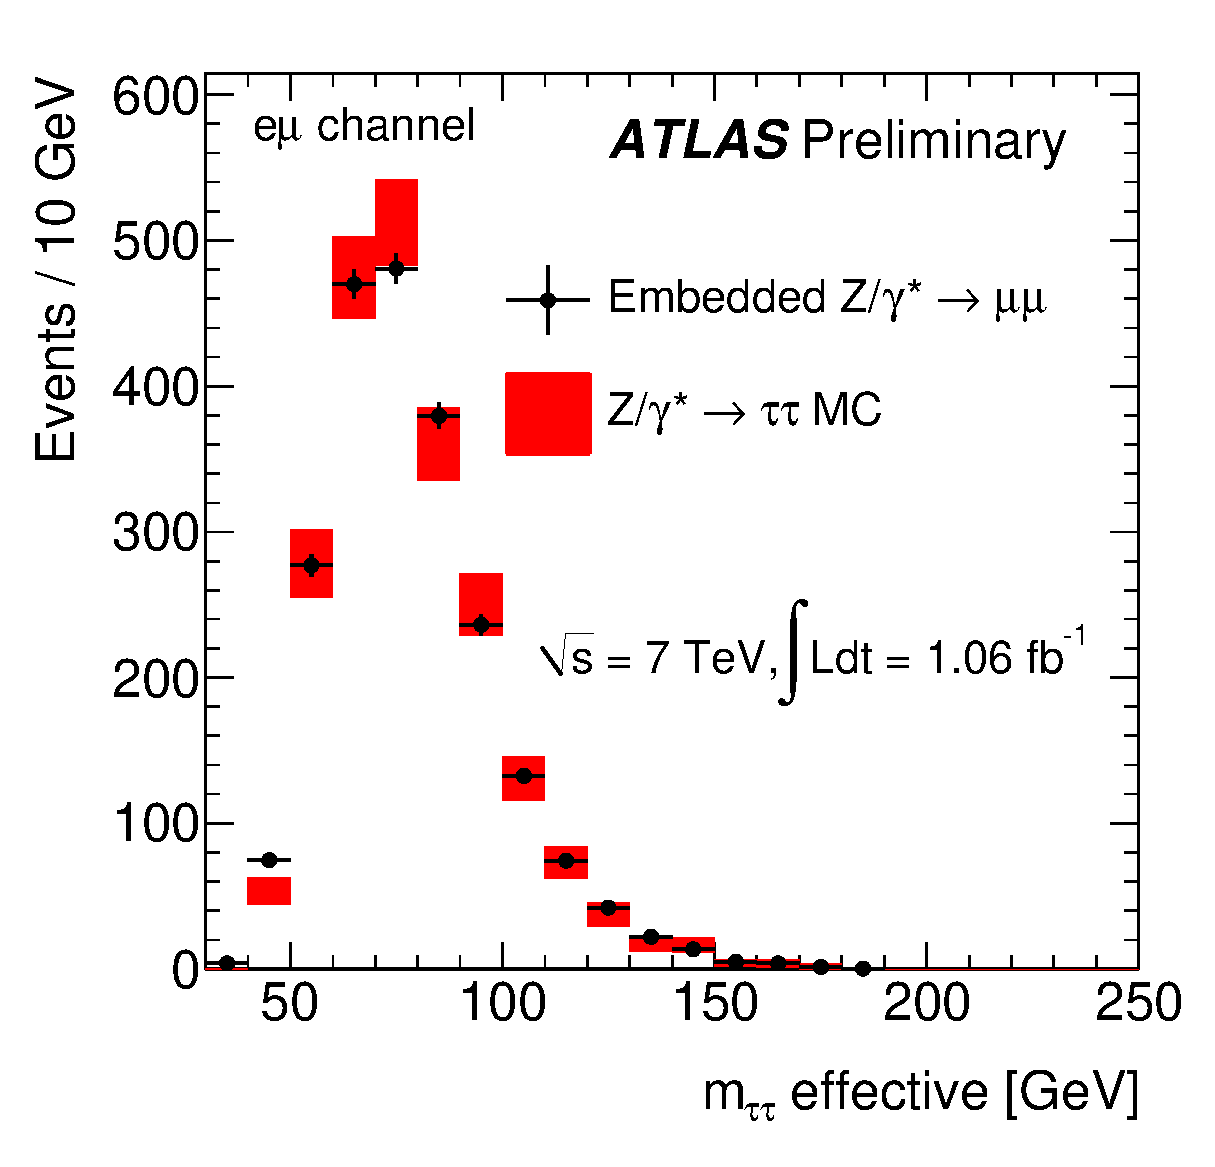
\includegraphics[width=0.48\textwidth]{figures/PERF-2013-06/fig_02a}
  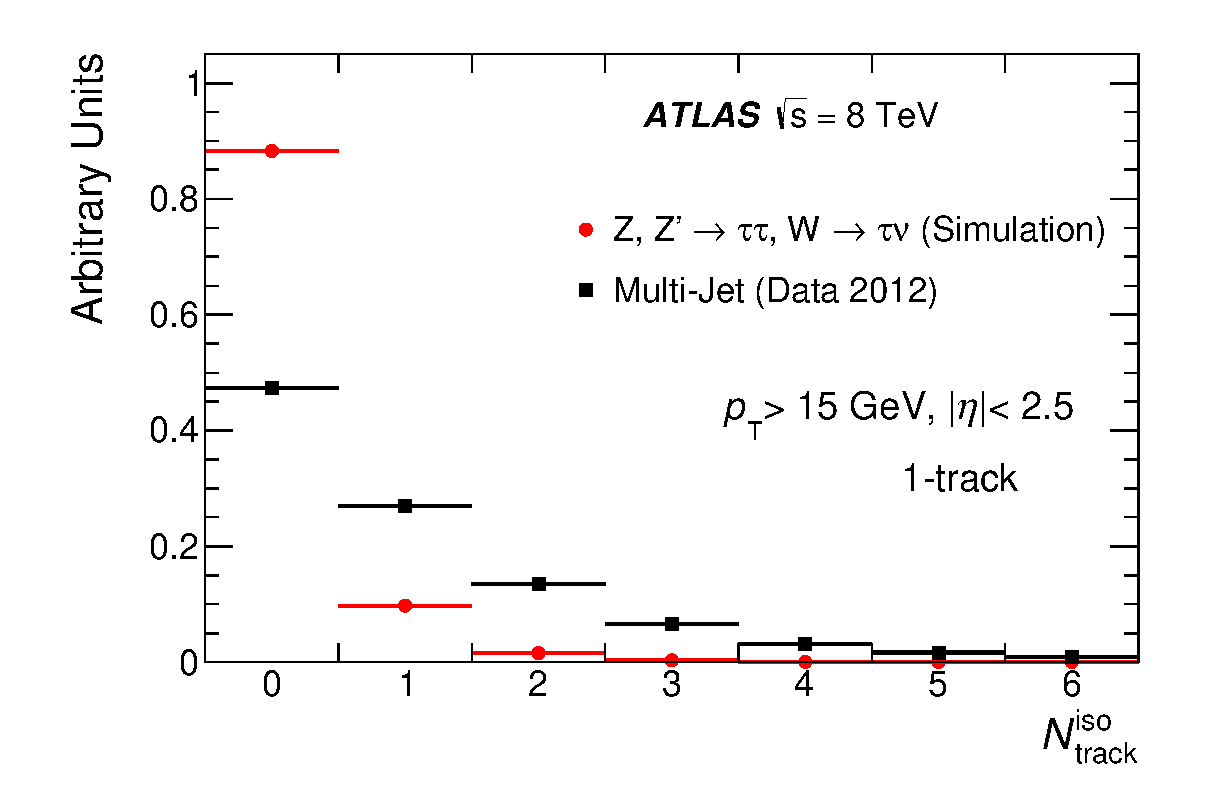
\includegraphics[width=0.48\textwidth]{figures/PERF-2013-06/fig_02b}
  \caption{Variables.}
  \label{fig:taus-id1p}
\end{figure}

\begin{figure}[tp]
  \centering
  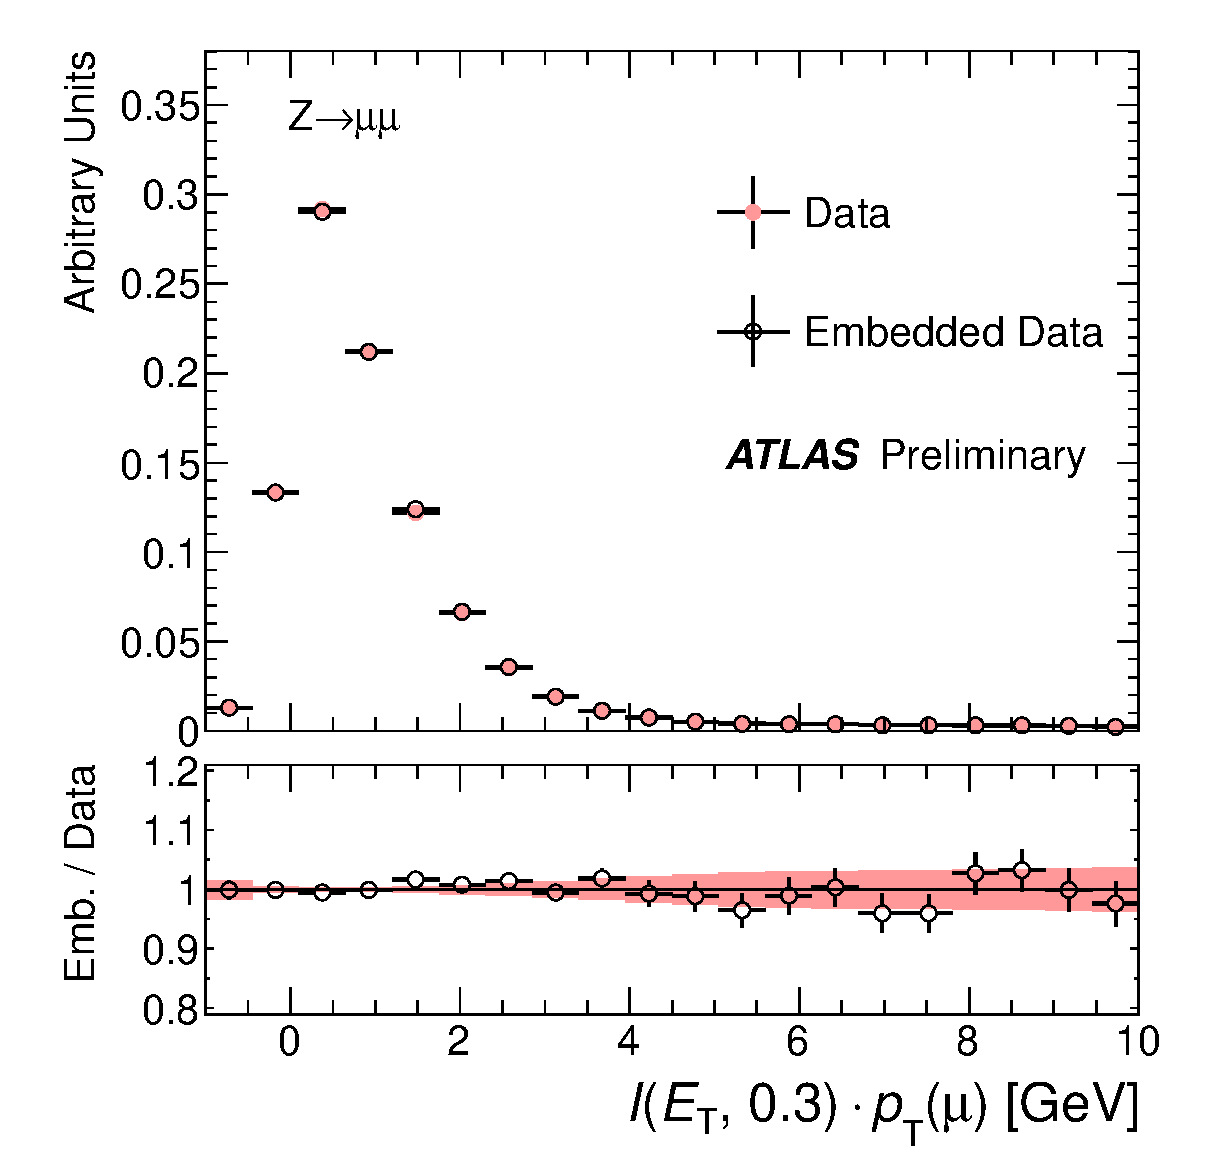
\includegraphics[width=0.48\textwidth]{figures/PERF-2013-06/fig_03a}
  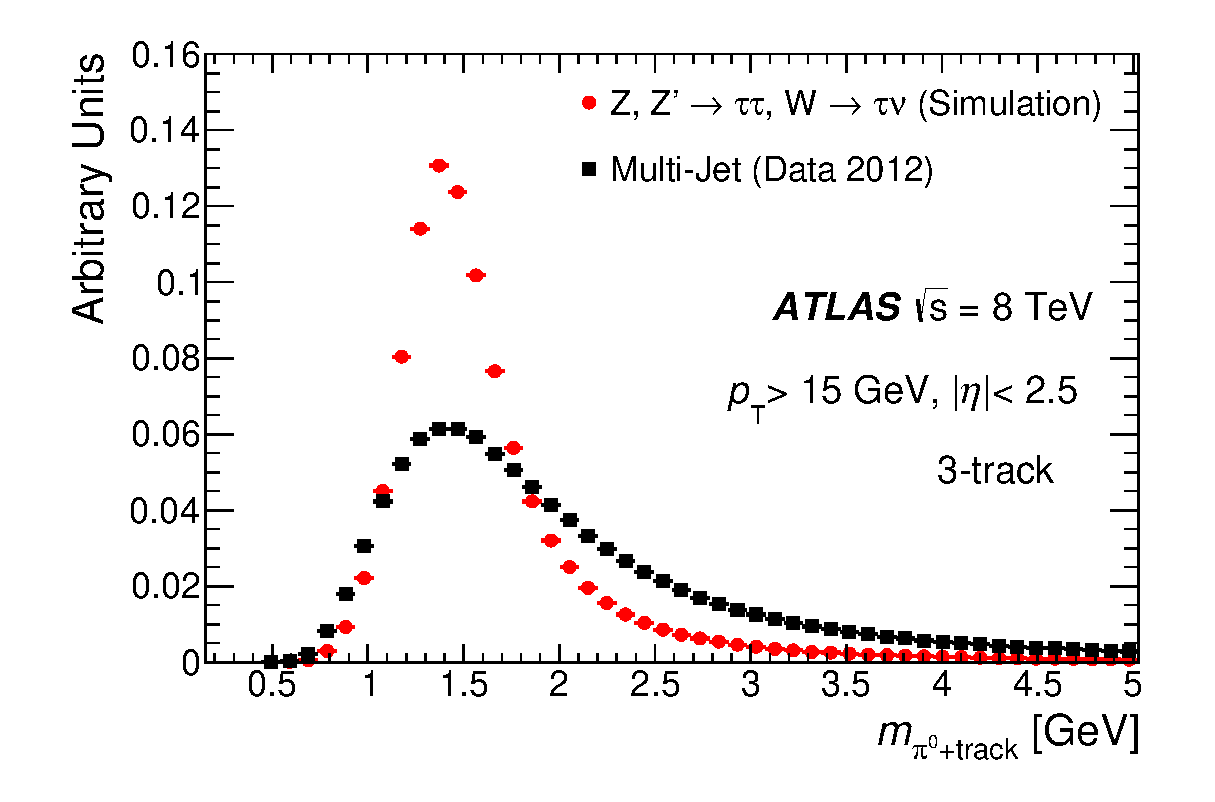
\includegraphics[width=0.48\textwidth]{figures/PERF-2013-06/fig_03b}
  \caption{Variables.}
  \label{fig:taus-id3p}
\end{figure}

\begin{figure}[tp]
  \centering
  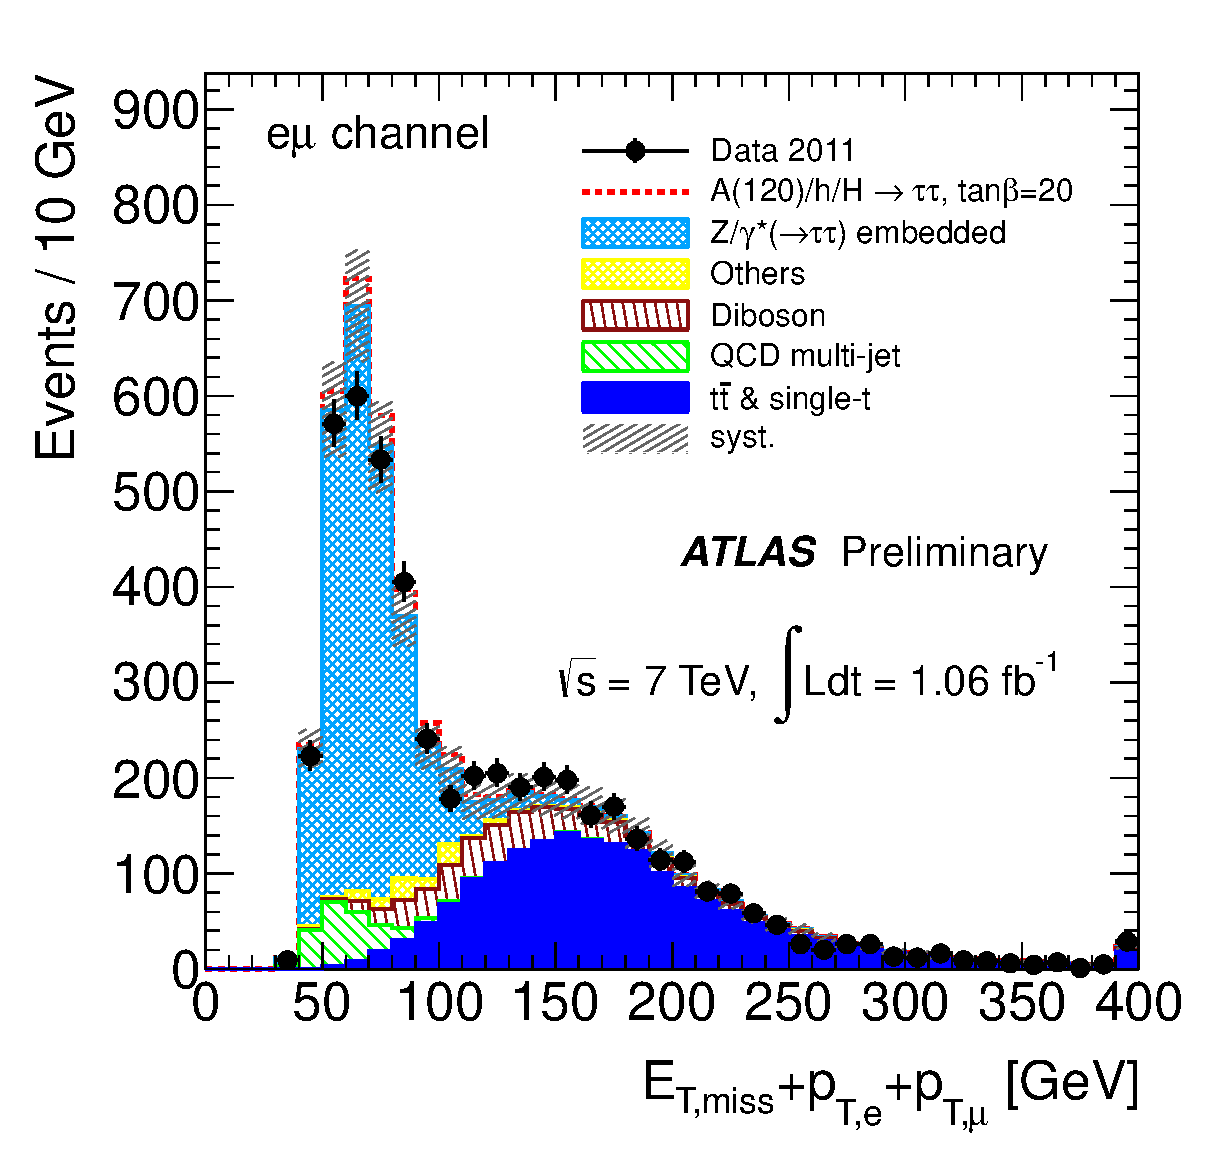
\includegraphics[width=0.48\textwidth]{figures/PERF-2013-06/fig_05a}
  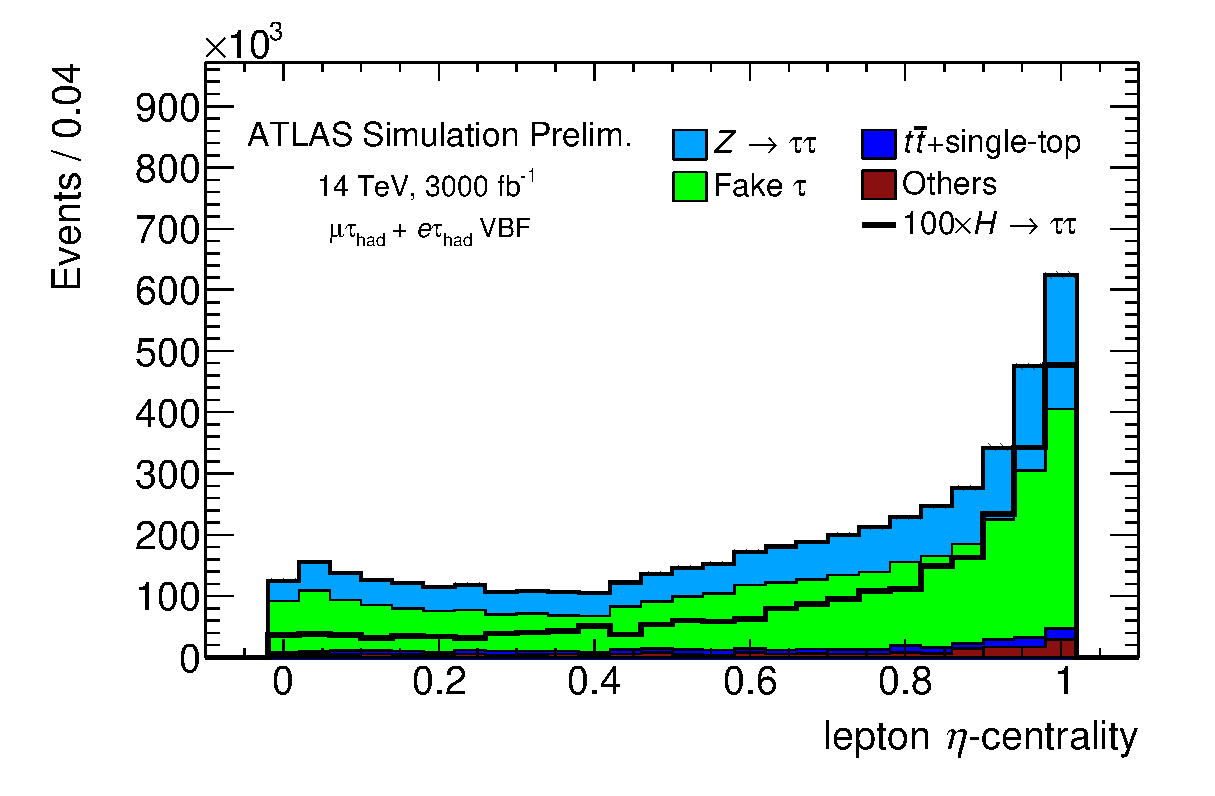
\includegraphics[width=0.48\textwidth]{figures/PERF-2013-06/fig_05b}
  \caption{Variables.}
  \label{fig:taus-idroc}
\end{figure}

\section{Leptons mis-identified as $\tauh$}
\label{sec:taus-leptonfakes}

\begin{figure}[tp]
  \centering
  \includegraphics[width=0.48\textwidth]{figures/tauperformance/muonfakes_mll}
  \includegraphics[width=0.48\textwidth]{figures/tauperformance/muonfakes_eta}
  \caption{Variables.}
  \label{fig:taus-muonfakes1}
\end{figure}

\begin{figure}[tp]
  \centering
  \includegraphics[width=0.48\textwidth]{figures/tauperformance/muonfakes_mlly}
  \includegraphics[width=0.48\textwidth]{figures/tauperformance/muonfakes_dR}
  \caption{Variables.}
  \label{fig:taus-muonfakes2}
\end{figure}

\begin{figure}[tp]
  \centering
  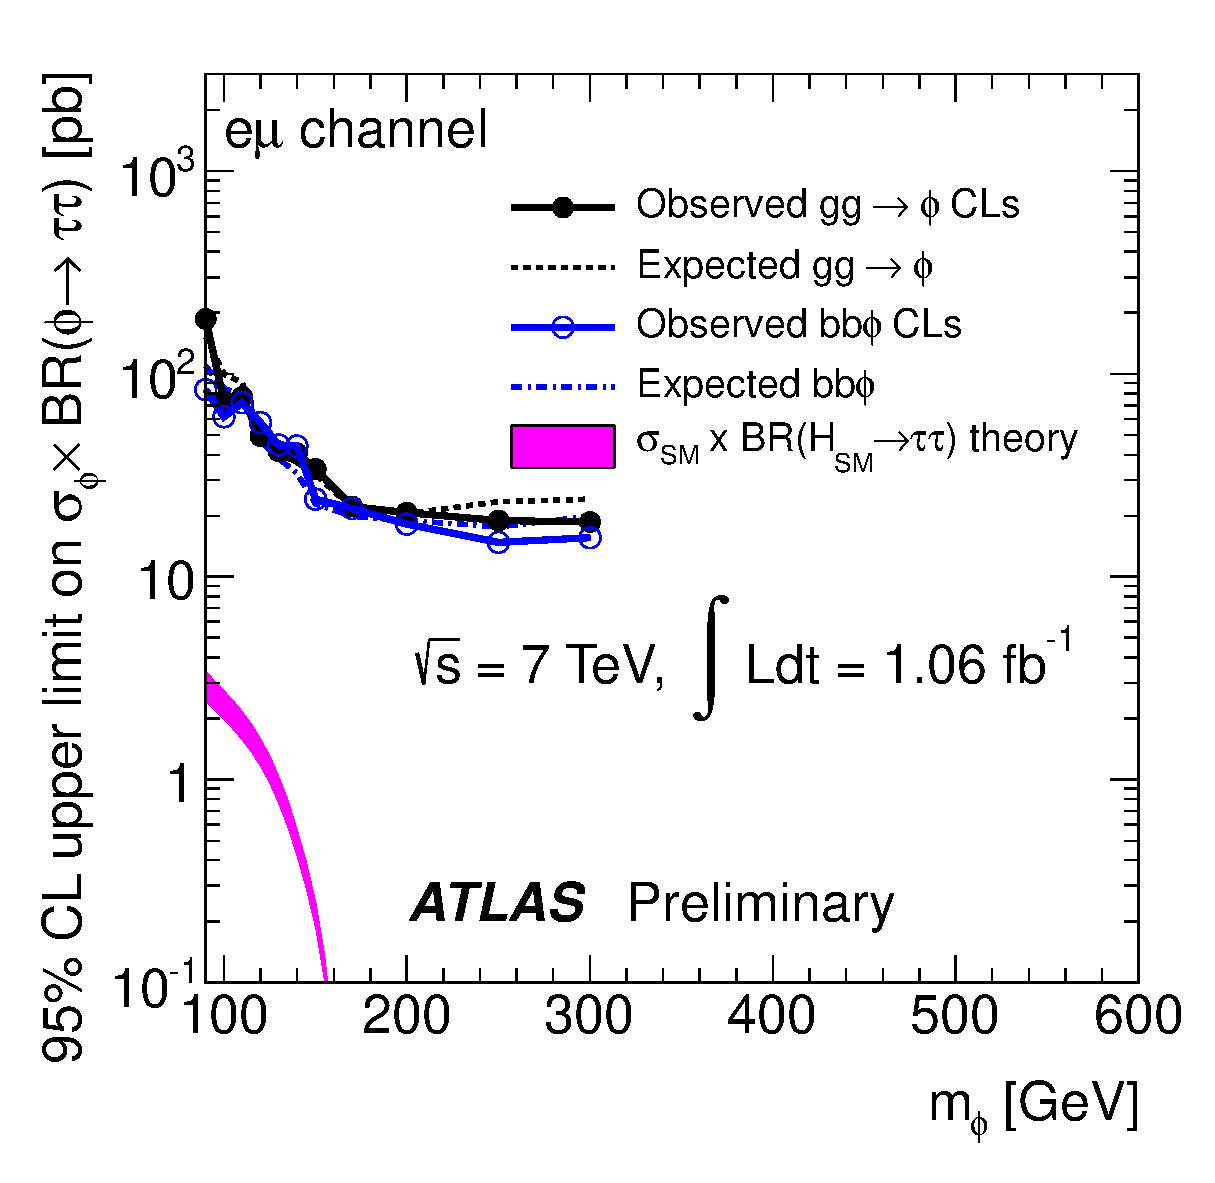
\includegraphics[width=0.48\textwidth]{figures/PERF-2013-06/fig_08a}
  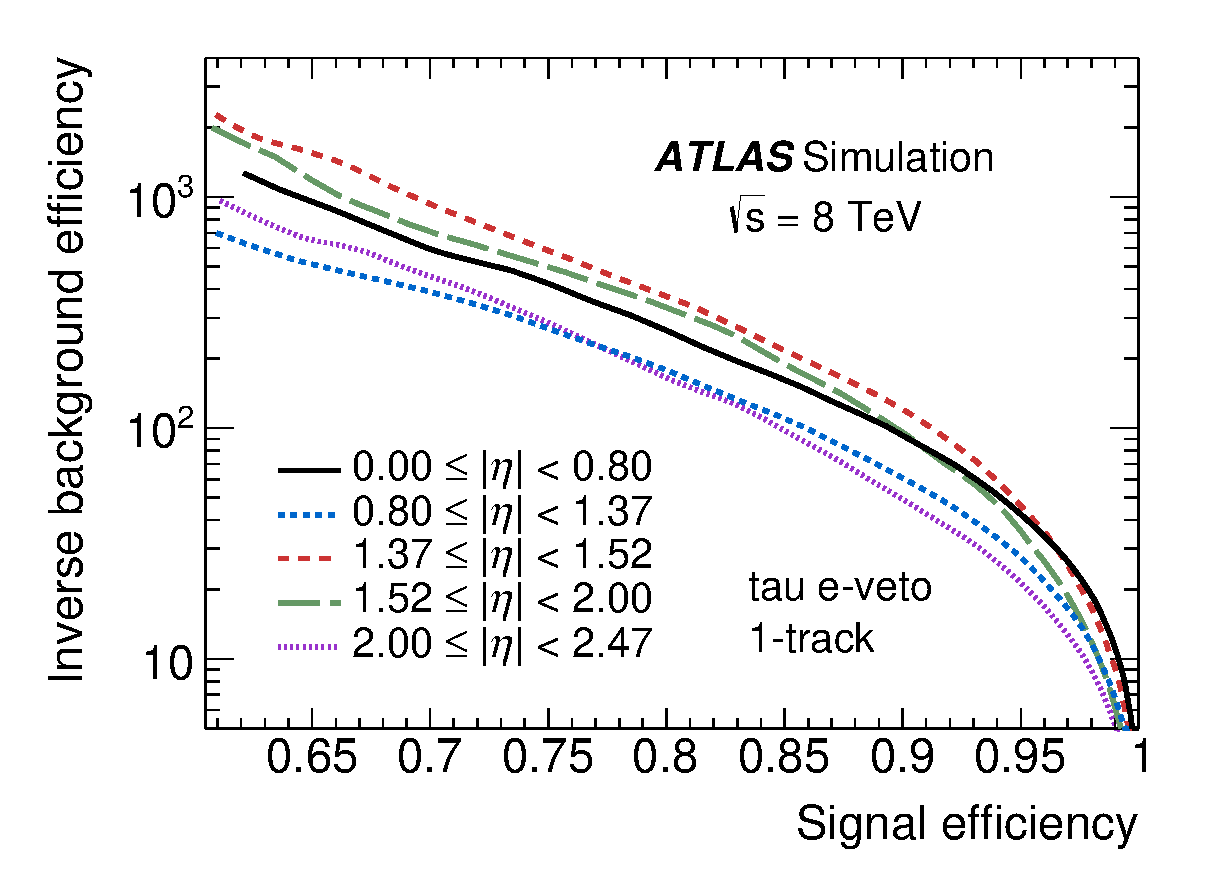
\includegraphics[width=0.48\textwidth]{figures/PERF-2013-06/fig_09}
  \caption{Variables.}
  \label{fig:taus-electronfakes1}
\end{figure}

\begin{figure}[tp]
  \centering
  \includegraphics[width=0.48\textwidth]{figures/PERF-2013-06/fig_14a}
  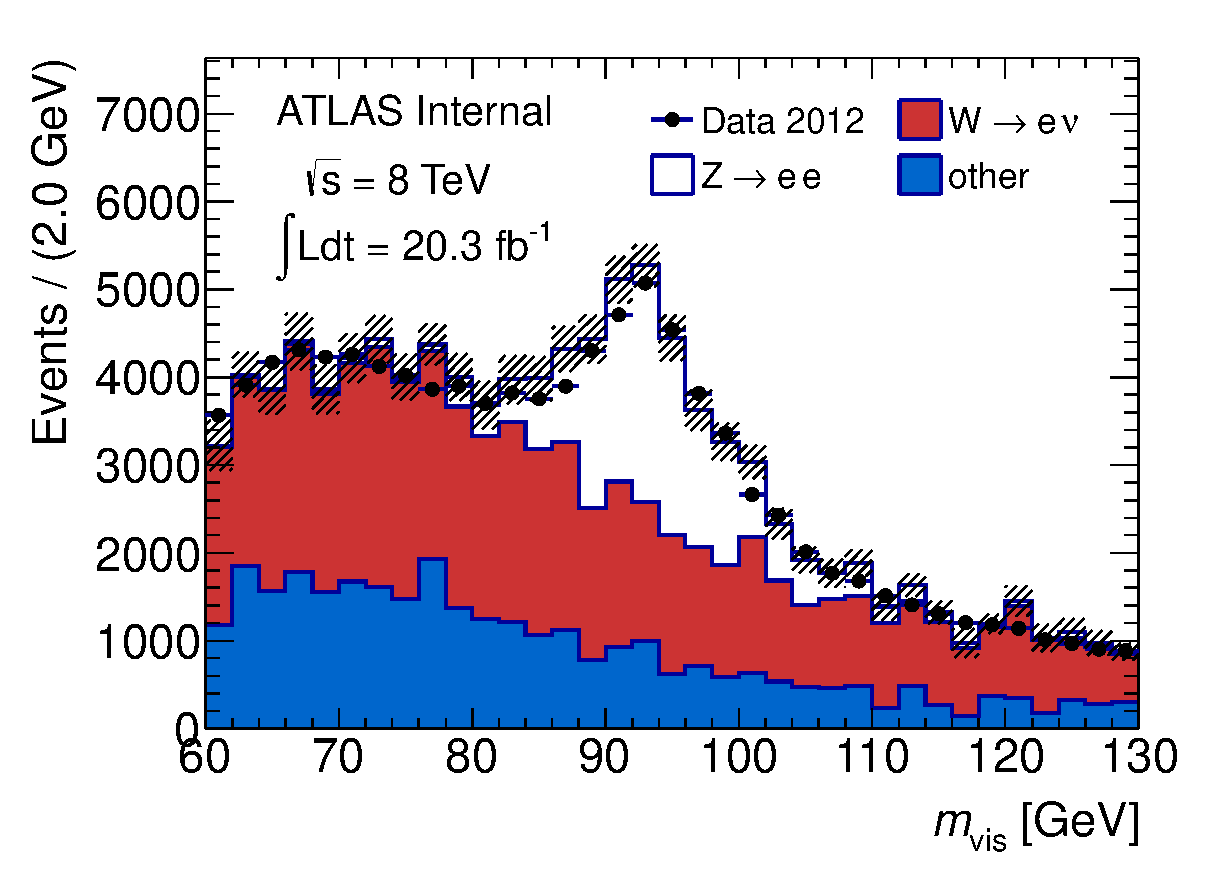
\includegraphics[width=0.48\textwidth]{figures/PERF-2013-06/eveto_mvis_mediumID_loosePPOLR_looseeveto}
  \caption{Variables.}
  \label{fig:taus-electronfakes2}
\end{figure}


